\documentclass[10pt,aspectratio=169]{beamer}

\usetheme[progressbar=foot]{metropolis}
\AtBeginSection{}

\usepackage{appendixnumberbeamer}
\usepackage{booktabs}
\usepackage{tabularx}
\usepackage{tikz}
\usetikzlibrary{arrows.meta,positioning,shapes.geometric}
\usepackage{xspace}
\usepackage{graphicx}
\usepackage[
  backend=biber,
  style=authoryear
]{biblatex}
\setbeamertemplate{bibliography item}{}
\addbibresource{bibliography.bib}

%................................................................................
% COLORS

\definecolor{ukudlaBlue}{RGB}{41, 60, 135}
\definecolor{ukudlaLightBlue}{RGB}{212, 216, 231}
\definecolor{ukudlaRed}{RGB}{164, 28, 34}
\definecolor{ukudlaLightRed}{RGB}{236, 209, 210}
\definecolor{ukudlaGreen}{RGB}{59, 139, 71}
\definecolor{ukudlaLightGreen}{RGB}{215, 231, 218}
\definecolor{ukudlaYellow}{RGB}{239, 198, 44}
\definecolor{ukudlaLightYellow}{RGB}{251, 243, 212}
\definecolor{white}{RGB}{255, 255, 255}
\definecolor{black}{RGB}{0, 0, 0}

\setbeamercolor{palette primary}{fg=white, bg=ukudlaGreen}
\setbeamercolor{progress bar}{fg=ukudlaRed, bg=ukudlaYellow}
\setbeamercolor{title separator}{fg=ukudlaRed, bg=ukudlaYellow}
\setbeamercolor{progress bar in head/foot}{fg=ukudlaRed, bg=ukudlaYellow}
\setbeamercolor{progress bar in section page}{fg=ukudlaRed, bg=ukudlaYellow}
\setbeamercolor{background canvas}{bg=white}
\setbeamercolor{block body}{bg=ukudlaLightGreen,fg=black}

%................................................................................
% PRESENTATION INFORMATION

\title{UKUDLA Data Science Certificate}
\subtitle{Introduction to Data Science for Food Systems Analysis}
\author{Markus Mößler}
\institute{University of Hohenheim}

%................................................................................
% CUSTOM FOOTER

\makeatletter
\setbeamertemplate{progress bar in head/foot}{%
  \tikzset{metropolis@progressbar@foreground/.style={fill=ukudlaGreen}}%
  \tikzset{metropolis@progressbar@background/.style={fill=ukudlaLightGreen}}%
  \begin{tikzpicture}[overlay, x=\paperwidth, y=1cm]
    \fill[metropolis@progressbar@background] (0,0) rectangle (1,0.10);
    \fill[metropolis@progressbar@foreground] (0,0) rectangle
      ({\insertframenumber/\inserttotalframenumber},0.10);
    \node[anchor=south west, yshift=0.25cm, xshift=0.2cm] at (0,0)
      {\includegraphics[height=0.75cm]{./logos/UKUDLA_logo_03_white_bg.pdf}};
    % current section
    \ifnum\value{section}>0
      \node[
        anchor=south east,
        yshift=0.22cm,
        xshift=-0.60cm,
        fill=ukudlaLightGreen,
        rounded corners=2pt,
        inner xsep=6pt,
        inner ysep=3pt,
        font=\scriptsize\bfseries,
        text=ukudlaRed
      ] at (1,0) {
        \insertsectionhead
      };
    \fi

  \end{tikzpicture}%
}
\makeatother

%................................................................................
% CUSTOM TITLE PAGE

\makeatletter
\setbeamertemplate{title page}{
  \begin{beamercolorbox}[sep=8pt,center,wd=\paperwidth,ht=0.5\paperheight]{title page top}
    \begin{minipage}[c]{1.00\textwidth}
      \raggedleft
      \includegraphics[height=1.00cm]{./logos/ukudla_universities.pdf}
      \vspace*{0.2cm}
    \end{minipage}
    \begin{beamercolorbox}[wd=0.9\paperwidth,sep=12pt,left]{top box}
      {\usebeamerfont{title}\usebeamercolor[fg]{title}\inserttitle\par}
      \vskip0.1cm
      {\usebeamerfont{subtitle}\usebeamercolor[fg]{subtitle}\insertsubtitle\par}
    \end{beamercolorbox}
  \end{beamercolorbox}
  \begin{beamercolorbox}[sep=8pt,center,wd=\paperwidth,ht=0.5\paperheight]{title page bottom}
    \begin{beamercolorbox}[wd=0.9\paperwidth,sep=12pt,left]{bottom box}
      \hbox{%
        \hspace*{1em}
        \begin{minipage}[c]{0.40\textwidth}
          \vskip1.0cm
          {\usebeamerfont{author}\usebeamercolor[fg]{author}\insertauthor\par}
          \vskip0.1cm
          {\usebeamerfont{institute}\usebeamercolor[fg]{institute}\insertinstitute\par}
        \end{minipage}%
        \hspace*{1.5cm}
        \begin{minipage}[c]{1.00\textwidth}
          \includegraphics[height=2.0cm]{./logos/UKUDLA_logo_05.pdf}
        \end{minipage}%
      }
    \end{beamercolorbox}
    \begin{minipage}[r]{1.00\textwidth}
      \centering
      \includegraphics[width=1.00\textwidth]{./logos/ukudla_sponsors.pdf}
    \end{minipage}
  \end{beamercolorbox}
}
\makeatother

\setbeamercolor{title page top}{bg=white}
\setbeamercolor{top box}{bg=ukudlaGreen}
\setbeamercolor{title page bottom}{bg=white}
\setbeamercolor{bottom box}{bg=ukudlaLightGreen}
\setbeamercolor{title}{fg=white}
\setbeamercolor{subtitle}{fg=white}
\setbeamercolor{author}{fg=black}
\setbeamercolor{institute}{fg=black}

%................................................................................
% DOCUMENT

\begin{document}

\maketitle

%--------------------------------------------------
{
\setbeamertemplate{frame numbering}[none]
\begin{frame}[noframenumbering]{Table of contents}
  \small
  \setbeamertemplate{section in toc}[sections numbered]
  \tableofcontents[hideallsubsections]
\end{frame}
}
%--------------------------------------------------

\section{Purpose}

%--------------------------------------------------
% CONTENT SLIDE 1/10
\begin{frame}{Why data science matters for food systems}
\small
\begin{columns}[T]
\column{0.47\textwidth}
\textbf{Food systems generate diverse evidence}
\begin{itemize}
  \item laboratory measurements and assays;
  \item designed field experiments;
  \item field observations, surveys and qualitative evidence; and
  \item administrative, market, climate and remote-sensing data.
\end{itemize}
\column{0.47\textwidth}
\textbf{Decisions require more than data}
\begin{itemize}
  \item transparent questions and assumptions;
  \item appropriate preparation and analysis;
  \item reproducible computational workflows; and
  \item careful interpretation of uncertainty.
\end{itemize}
\end{columns}
\vspace{0.35cm}
\begin{beamercolorbox}[rounded=true,sep=9pt]{block body}
Data science connects questions, data, computation and judgment to produce evidence that can be inspected and reused.
\end{beamercolorbox}
\end{frame}
%--------------------------------------------------

%--------------------------------------------------
% CONTENT SLIDE 2/10
\begin{frame}{The challenge is a chain of decisions}
\small
\centering
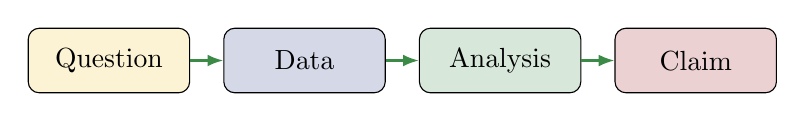
\begin{tikzpicture}[
  workflowstep/.style={draw,rounded corners,minimum width=2.05cm,minimum height=0.82cm,align=center},
  arrow/.style={-{Latex[length=2mm]},thick,ukudlaGreen}
]
  \node[workflowstep,fill=ukudlaLightYellow] (question) {Question};
  \node[workflowstep,fill=ukudlaLightBlue,right=0.42cm of question] (data) {Data};
  \node[workflowstep,fill=ukudlaLightGreen,right=0.42cm of data] (analysis) {Analysis};
  \node[workflowstep,fill=ukudlaLightRed,right=0.42cm of analysis] (claim) {Claim};
  \draw[arrow] (question) -- (data);
  \draw[arrow] (data) -- (analysis);
  \draw[arrow] (analysis) -- (claim);
\end{tikzpicture}
\vspace{0.45cm}
\raggedright
\begin{itemize}
  \item Available data may not represent the intended population or concept.
  \item Transformations and models encode assumptions that affect conclusions.
  \item Results can be technically correct but scientifically misleading.
  \item Documentation and reproducibility make the decision chain reviewable.
\end{itemize}
\end{frame}
%--------------------------------------------------

\section{Data Science}

%--------------------------------------------------
% CONTENT SLIDE 3/10
\begin{frame}{Data science is an integrated practice}
\small
\begin{columns}[T]
\column{0.31\textwidth}
\centering
\textbf{Domain knowledge}

\scriptsize Defines meaningful questions, measurements and interpretations.
\column{0.31\textwidth}
\centering
\textbf{Statistical reasoning}

\scriptsize Describes variation, evaluates relationships and quantifies uncertainty.
\column{0.31\textwidth}
\centering
\textbf{Computing practice}

\scriptsize Acquires, transforms, analyzes and communicates data reproducibly.
\end{columns}
\vspace{0.65cm}
\begin{beamercolorbox}[rounded=true,sep=9pt]{block body}
No single tool defines data science. Credible work depends on how these forms of knowledge are combined.
\end{beamercolorbox}
\end{frame}
%--------------------------------------------------

%--------------------------------------------------
% CONTENT SLIDE 4/10
\begin{frame}{Different questions require different analyses}
\small
\begin{tabularx}{\textwidth}{lXX}
\toprule
\textbf{Purpose} & \textbf{Question} & \textbf{Example output} \\
\midrule
Descriptive & What patterns are present in the observed data? & Summaries, distributions and trends \\
Explanatory & How should an assumed relationship be estimated and interpreted? & Effect estimate with assumptions \\
Predictive & How accurately can an unknown outcome be predicted? & Out-of-sample predictions and error \\
\bottomrule
\end{tabularx}
\vspace{0.45cm}
\begin{itemize}
  \item A useful analysis begins with a clearly stated purpose.
  \item Explanatory and predictive success are not interchangeable.
  \item Every conclusion is conditional on data quality and design choices.
\end{itemize}
\end{frame}
%--------------------------------------------------

%--------------------------------------------------
% CONTENT SLIDE 5/10
\begin{frame}{A data science workflow is iterative}
\small
\centering
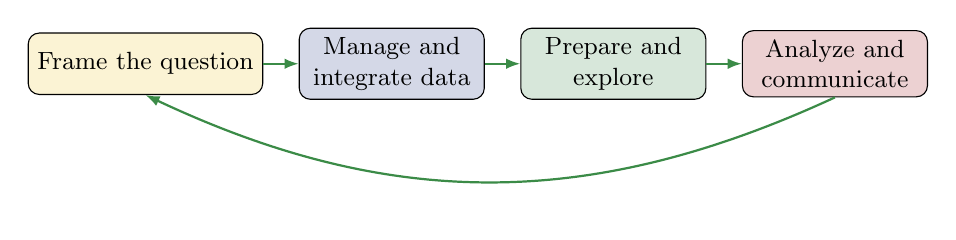
\begin{tikzpicture}[
  stage/.style={draw,rounded corners,minimum width=2.35cm,minimum height=0.78cm,align=center,font=\small},
  arrow/.style={-{Latex[length=1.8mm]},thick,ukudlaGreen}
]
  \node[stage,fill=ukudlaLightYellow] (frame) {Frame the question};
  \node[stage,fill=ukudlaLightBlue,right=0.45cm of frame] (manage) {Manage and\\integrate data};
  \node[stage,fill=ukudlaLightGreen,right=0.45cm of manage] (prepare) {Prepare and\\explore};
  \node[stage,fill=ukudlaLightRed,right=0.45cm of prepare] (analyse) {Analyze and\\communicate};
  \draw[arrow] (frame) -- (manage);
  \draw[arrow] (manage) -- (prepare);
  \draw[arrow] (prepare) -- (analyse);
  \draw[arrow,bend left=25] (analyse.south) to (frame.south);
\end{tikzpicture}
\vspace{0.55cm}
\raggedright
\begin{itemize}
  \item Findings often reveal new data-quality issues or better questions.
  \item Iteration is expected; undocumented iteration is the risk.
  \item Versioned inputs, code and decisions preserve the path to a result.
\end{itemize}
\end{frame}
%--------------------------------------------------

%--------------------------------------------------
% CONTENT SLIDE 6/10
\begin{frame}{Credibility requires reproducibility and responsibility}
\small
\begin{columns}[T]
\column{0.47\textwidth}
\textbf{Reproducible practice}
\begin{itemize}
  \item version code and documentation;
  \item record software environments;
  \item automate transformations; and
  \item preserve provenance and validation.
\end{itemize}
\column{0.47\textwidth}
\textbf{Responsible practice}
\begin{itemize}
  \item respect licenses, privacy and consent;
  \item examine representation and bias;
  \item distinguish evidence from assumptions; and
  \item communicate limitations honestly.
\end{itemize}
\end{columns}
\vspace{0.35cm}
\centering
\textcolor{ukudlaRed}{A result is credible only when its production and interpretation can be examined.}
\end{frame}
%--------------------------------------------------

\section{Course Structure}

%--------------------------------------------------
% CONTENT SLIDE 7/10
\begin{frame}{Part 1 builds tools for reproducible work}
\small
\begin{columns}[T]
\column{0.31\textwidth}
\centering
\textbf{Version control}

\scriptsize Record meaningful project states and collaborate through Git and GitHub.
\column{0.31\textwidth}
\centering
\textbf{Environments}

\scriptsize Recreate package and system dependencies with \texttt{renv} and Docker.
\column{0.31\textwidth}
\centering
\textbf{Remote computing}

\scriptsize Work safely on other computers through SSH and Linux tools.
\end{columns}
\vspace{0.65cm}
\begin{beamercolorbox}[rounded=true,sep=9pt]{block body}
These tools support every later topic; they are part of the analytical method, not administrative extras.
\end{beamercolorbox}
\end{frame}
%--------------------------------------------------

%--------------------------------------------------
% CONTENT SLIDE 8/10
\begin{frame}{Part 2 establishes trustworthy analytical data}
\small
\begin{columns}[T]
\column{0.31\textwidth}
\centering
\textbf{Data management}

\scriptsize Describe, organize, validate and preserve data and their history.
\column{0.31\textwidth}
\centering
\textbf{Data integration}

\scriptsize Align identifiers, time, space and meaning across sources.
\column{0.31\textwidth}
\centering
\textbf{Data preparation}

\scriptsize Transform managed data into an explicit unit of analysis.
\end{columns}
\vspace{0.65cm}
\begin{beamercolorbox}[rounded=true,sep=9pt]{block body}
Analytical validity begins before modeling: later results inherit the choices made in constructing the data.
\end{beamercolorbox}
\end{frame}
%--------------------------------------------------

%--------------------------------------------------
% CONTENT SLIDE 9/10
\begin{frame}{Part 3 develops complementary forms of analysis}
\small
\begin{tabularx}{\textwidth}{lX}
\toprule
\textbf{Topic} & \textbf{Primary role} \\
\midrule
Data visualization & Reveal structure and communicate evidence through graphical encodings \\
Descriptive analysis & Summarize distributions, dependence, change and stability \\
Explanatory analysis & Estimate and qualify relationships under causal assumptions \\
Predictive analysis & Evaluate forecasts on observations not used for model fitting \\
\bottomrule
\end{tabularx}
\vspace{0.45cm}
\begin{itemize}
  \item Each topic combines motivation, reusable concepts and application guidance.
  \item Detailed pages support study; the example repository supports practice.
\end{itemize}
\end{frame}
%--------------------------------------------------

\section{Key Message}

%--------------------------------------------------
% CONTENT SLIDE 10/10
\begin{frame}{Key message: make the complete reasoning chain visible}
\large
\begin{beamercolorbox}[rounded=true,sep=11pt]{block body}
Data science is the disciplined construction of evidence from questions, data, computation and assumptions—not merely the use of software or models.
\end{beamercolorbox}
\vspace{0.45cm}
\small
\begin{itemize}
  \item Start with the purpose of the analysis.
  \item Treat data and computational choices as part of the evidence.
  \item Match descriptive, explanatory or predictive methods to the question.
  \item Preserve enough information for others to inspect, reproduce and reuse the work.
\end{itemize}
\end{frame}
%--------------------------------------------------

%--------------------------------------------------
\begin{frame}[plain,noframenumbering]{Supported by}
  South African government and the National Research Foundation
  \begin{flushleft}
    \includegraphics[width=0.50\textwidth]{./logos/ukudla_south_african_sponsors.pdf}
  \end{flushleft}
  German government and the German Academic Exchange Service
  \begin{flushleft}
    \includegraphics[width=1.00\textwidth]{./logos/ukudla_german_sponsors.pdf}
  \end{flushleft}
\end{frame}
%--------------------------------------------------

\end{document}
